\chapter{Propostas para a mellora da seguridade}
\minitoc
\clearpage

\section{Contedores correndo sobre \gls{MV}s}

As \gls{MV}s son consideradas máis seguras que os contedores xa que engaden unha capa extra de illamento entre as aplicacións e a máquina anfitrioa. Unha aplicación correndo dentro dunha \gls{MV}, soamente é quen de comunicarse co \textit{kernel} da propia \gls{MV}, mais non co \textit{kernel} da máquina anfitrioa \cite{Securing-Docker-Containers-from-Denial-of-Service}. Amais, unha vez comprometido o \textit{kernel} da máquina virtual, tamén habería que conseguir traspasar a capa que supón o hipervisor, constituíndo un modelo con dúas capas extra de seguridade en comparativa cos contedores \cite{state-of-art-docker-security}.\\

Pola contra, os contedores pódense comunicar directamente co \textit{kernel} da máquina anfitrioa, permitindo así a un posíbel atacante gañar enormes privilexios na mesma se o seu ataque ten éxito.\\

Un posíbel fornecemento da seguridade do sistema podería pasar pola emprega dun sistema híbrido no que se despregaran contedores nunha \gls{MV}. Deste xeito, un grupo enteiro de servizos quedarían illados dos outros, ao estaren executándose dentro de dita \gls{MV}. Así, os contedores contarían coas capas extra de seguridade aportadas polas \gls{MV}s, comunicándose co seu \textit{kernel} e non directamente co \textit{kernel} da máquina anfitrioa. En troques, perderíamos a eficiencia que estes nos aportan, aínda que manteríamos intactas as súas cualidades de despregamento lixeiro e portabilidade. Outra característica moi a ter en conta no entorno no que se desenvolve este traballo é a posibilidade de continuar empregando eficientemente servizos de computación de alta prestacións, como a utilización total da memoria ou da CPU, a emprega da rede InfiniBand ou da GPU, servizos hardware aos que non se pode ter acceso directo coa emprega de \gls{MV}s.

\section{Aplicación de capas externas de seguridade}

Ademais das características de seguridade xa implantadas polas propias tecnoloxías de contedorización, ou que relegan en capacidades do \textit{kernel} de Linux, é posíbel engadir unha capa extra de seguridade empregando sistemas ben coñecidos enfocados na seguridade e con compatibilidade con contedores. Por exemplo, podemos facer emprega de mecanismos de control de acceso como o modelo discrecional, \textit{Discretionary Access Control} (DAC), ou o obrigatorio, \textit{Mandatory Access Control} (\gls{MACC}).\\

Facendo unha breve introdución, a misión dos controis de acceso é asegurar que os usuarios correctos posúen os privilexios adecuados, para o que fan uso de suxeitos, obxectos e privilexios.

\subsection{Modelo centralizado: \gls{MACC} e \gls{SELinux}}

\gls{MACC} constitúe unha implantación dun mecanismo de control de acceso obrigatorio (\gls{MACC}), Seguridade de múltiples niveis e seguridade de múltiples categorías (MLS) no \textit{kernel} de Linux. O proxecto \textit{sVirt} baséase en \gls{SELinux} e intégrase con Libvirt para provir unha separación segura para os contedores, xa que evita que os procesos raíz dentro dun contedor infiran cos procesos que se executan fóra deste contedor. \cite{Securing-Docker-Containers-from-Denial-of-Service}\\

Este modelo basea o seu funcionamento en políticas do sistema que non poden ser alteradas por usuarios individuais. Neste modelo, os obxectos inclúen un nivel de seguridade e un conxunto de categorías, mentres que os usuarios posúen permisos para cada clase. Deste xeito, existen regras baseadas en clases de acceso e autorización para administrar a lectura e escritura de obxectos. \\

Co fin de reducir a exposición de seguridade e cumprir co principio do mínimo privilexio, moitos sistemas operativos proporcionan un sistema \gls{MACC} integrado. Os \gls{MACC} poden ser empregados para fornecer o illamento entre os diferentes contedores e a máquina anfitrioa, así como para cumprir as políticas dos procesos executados dentro dos contedores \cite{OS-level-security}. Dita característica está completamente integrada no \textit{kernel}, mais debido ás complexas regras que o conforman, pode ser difícil de configurar. Algunhas das solucións máis comúns para a súa emprega son AppArmor e \gls{SELinux} \cite{TFM}.\\

Nos sistemas que empregan \gls{SELinux}, Docker aproveita a política definida no proxecto \textit{sVirt}, no que se apuntan políticas de seguridade para diferentes modelos de virtualización. Existen dúas maneiras de separar os procesos en \gls{SELinux}:

\begin{enumerate}
    \item \textit{Type Enforcement} (TE): unha etiqueta que contén un tipo está asociada a cada suxeito (proceso) e obxecto do sistema (ficheiro e directorio). A política define as accións permitidas entre os tipos e o \textit{kernel} impón estritamente estas regras. Docker asigna unha etiqueta cun conxunto reducido de privilexios a todos os procesos que se executan en contedores. TE emprégase para protexer o motor de Docker e a máquina anfitrioa dos contedores, que poden provir de fontes que non sexan de confianza.
    
    \item \textit{Multi-Category Secutiry} (MCS): a etiqueta asignada ao suxeito ou obxecto pódese subdividir con múltiples categorías para crear instancias diferentes do mesmo tipo. Acéptase unha solicitude de acceso se TE o permite primeiro e o suxeito e o obxecto están na mesma categoría. Non obstante, é vantaxoso se se asignan diferentes categorías a diferentes contedores para que teñan unha separación clara entre si.
\end{enumerate}

Podemos concluír que \gls{SELinux} supón unha capa engadida de seguridade que protexe o sistema da máquina anfitrioa, polo que no caso de que un ataque tivese éxito no interior dun contedor e conseguise acceder á propia máquina anfitrioa, \gls{SELinux} interviría para frustrar o ataque. Se un proceso de dentro do contedor consegue obter acceso a un arquivo da máquina anfitrioa e tenta facer operación de lectura ou escritura, \gls{SELinux} encargarase antes de verificar o seu acceso, impedindo o ataque ao detectar a falta de tales privilexios. \cite{SELinuxMitigates}

\section{Actualización do sistema}
\label{actualizacionSistema}

Unha das premisas máis importantes no eido da seguridade parte de manter o noso sistema ao día, para obter os parches de seguridade actuais e pór solución a un gran número de vulnerabilidades. Cando traballamos con contedores, esta premisa mantense presente, e grazas á flexibilidade que estes nos outorgan, debemos manter sempre o sistema actualizado para diminuír o número de vulnerabilidades que poidan conter.\\

Para evidenciar tal afirmación, realizarase unha proba con contedores Docker e Clair. O desenvolvemento esperado da proba é o seguinte:

\begin{enumerate}
    \item Descarga dunha imaxe dun contedor dende o Docker Hub.
    \item Exploración do número de vulnerabilidades existentes en dita imaxe coa axuda de Clair.
    \item Creación dun repositorio propio no Docker Hub, onde se almacenará unha imaxe derivada da imaxe orixinal.
    \item Actualización do sistema atopado no contedor, coa axuda do xestor de paquetes \gls{APT}.
    \item Creación da imaxe derivada, mediante a realización dun \textit{commit} sobre o contedor coas actualizacións xa efectuadas.
    \item Exploración do número de vulnerabilidades existentes na imaxe derivada e actualizada.
\end{enumerate}

Posto que xa existen imaxes no sistema, será empregada unha delas. Concretamente será empregada unha imaxe de MongoDB. Se comezamos facendo a primeira análise con \textit{clair-scanner} (figura \ref{rep1}), vemos como atopamos en primeira instancia 73 vulnerabilidades. Posteriormente realizamos o proceso de inicio de sesión no Docker Hub (figura \ref{rep3}), no cal xa existirá un repositorio creado para o almacenamento da imaxe que imos formar a partir da imaxe de MongoDB oficial. Continuaremos coa actualización dos paquetes mediante \gls{APT} (figura \ref{rep4}). Tendo xa un contedor actualizado, realizaremos un \textit{commit} deste sobre a nosa propia imaxe (figura \ref{rep5}). Para rematar, invocamos novamente á ferramenta \textit{clair-scanner}, mais está vez para que realice unha análise de vulnerabilidades sobre a imaxe derivada que acabamos de formar (figura \ref{rep2}). Desta segunda volta, a ferramenta detecta 66 vulnerabilidades, é dicir 7 vulnerabilidades menos no sistema con tan só realizar unha simple actualización. Queda por tanto, probada a importancia de manter o noso sistema ao día. Ademais, é probábel que se entramos nun estudo máis minucioso sexa posíbel reducir aínda máis o número de vulnerabilidades, por exemplo, eliminando librarías innecesarias, e conseguir así un sistema máis seguro.

\begin{figure}
\centerline{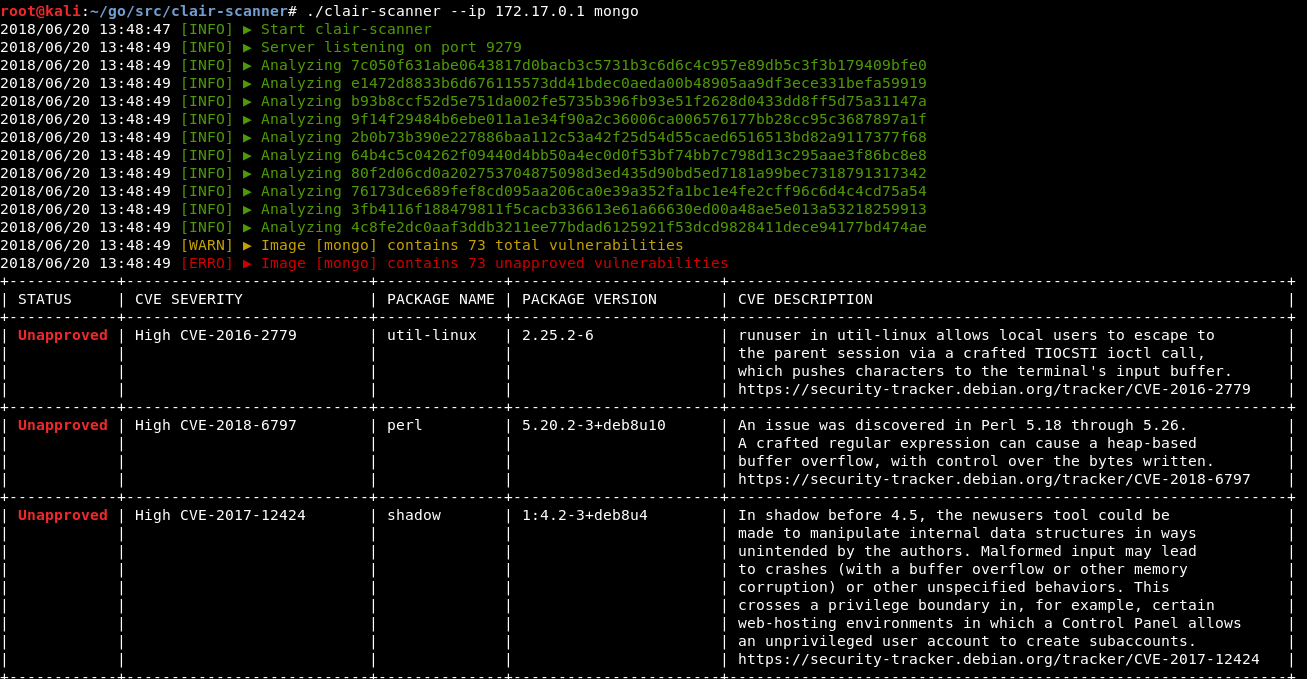
\includegraphics[width=15cm]{figuras/rep1.png}}
\caption{Escáner coa ferramenta \textit{clair-scanner} dunha imaxe de MongoDB}
\label{rep1}
\end{figure}

\begin{figure}
\centerline{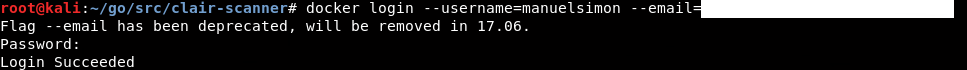
\includegraphics[width=15cm]{figuras/rep3.png}}
\caption{Inicio de sesión no Docker Hub}
\label{rep3}
\end{figure}

\begin{figure}
\centerline{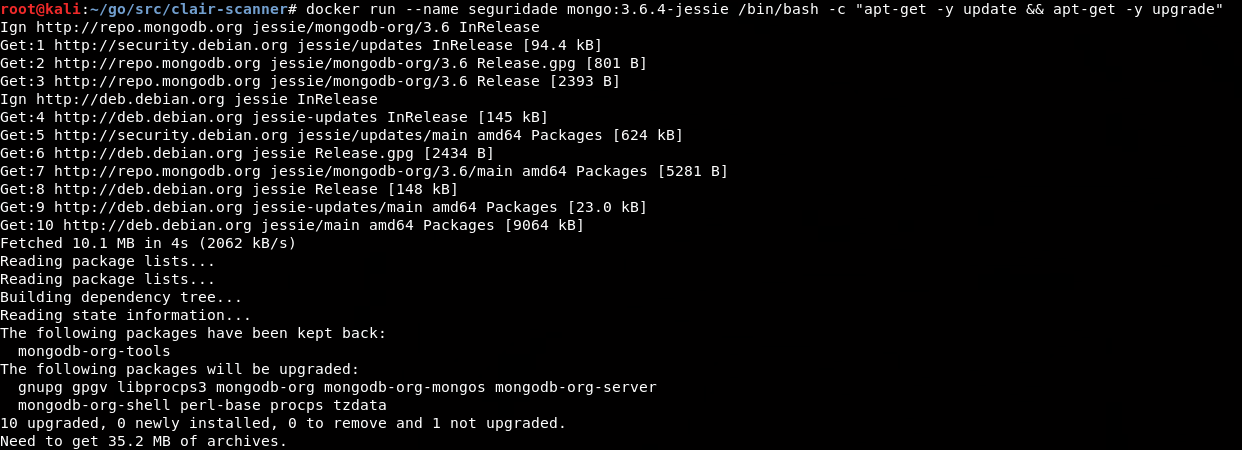
\includegraphics[width=15cm]{figuras/rep4.png}}
\caption{Execución do contedor ``seguridade'' a partir dunha imaxe de MongoDB e actualización dos paquetes}
\label{rep4}
\end{figure}

\begin{figure}
\centerline{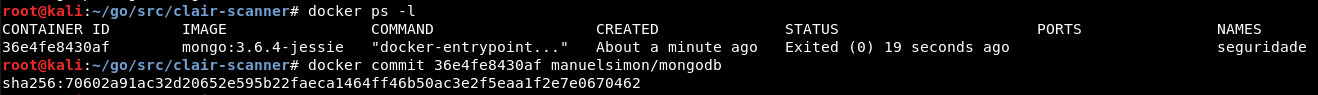
\includegraphics[width=15cm]{figuras/rep5.png}}
\caption{Execución de \textit{commit} do contedor ``seguridade'' sobre a nosa propia imaxe}
\label{rep5}
\end{figure}

\begin{figure}
\centerline{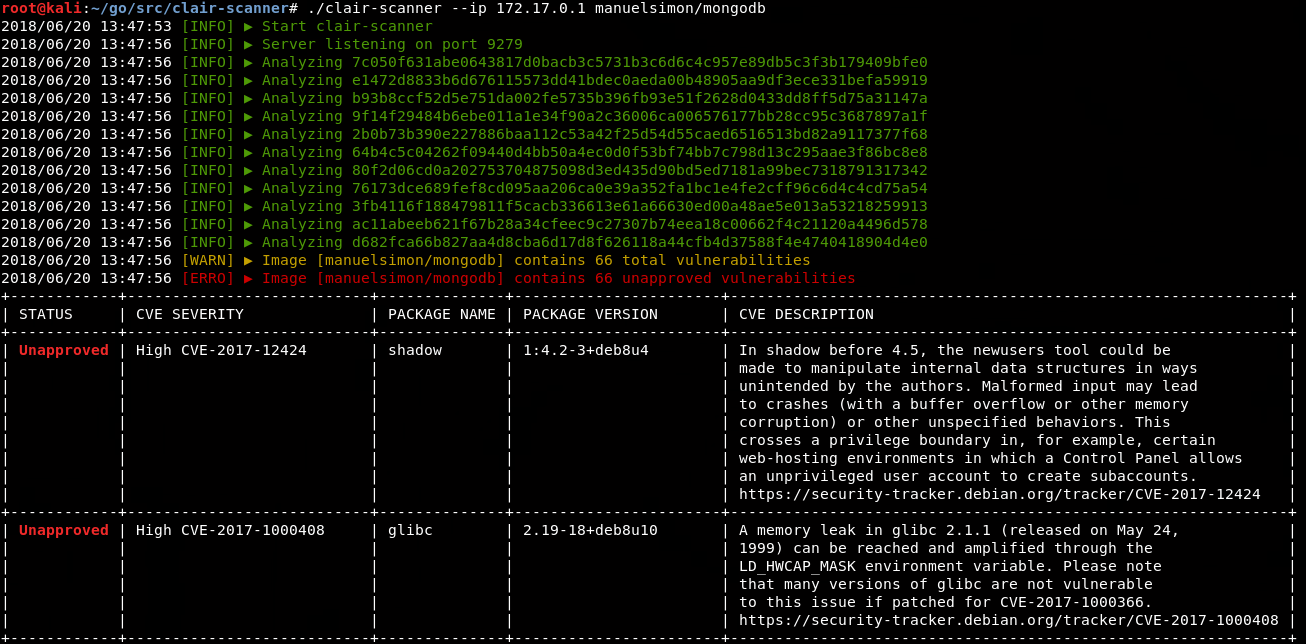
\includegraphics[width=15cm]{figuras/rep2.png}}
\caption{Escáner coa ferramenta \textit{clair-scanner} da imaxe actualizada de MongoDB}
\label{rep2}
\end{figure}

\section{Auditoría do sistema}

A auditoría informática é un proceso que consiste en recoller, agrupar e avaliar evidencias para determinar se un sistema posúe un nivel de seguridade adecuado, ou leva a cabo eficazmente os fins da organización, empregando eficientemente os recursos e cumprindo as leis e regulacións establecidas. A medida que as tecnoloxías de contedorización se van facendo un oco na industria, aparecen cada vez máis medidas reguladoras para a súa correcta utilización.\\

\subsection{\textit{Docker Bench Audit Tool}}
\label{DockerBeckAuditTool}

No eido da auditoría de seguridade na emprega de contedores podémonos atopar coa ferramenta \textit{Docker Bench Audit Tool}, facilitada polos propios desenvolvedores de Docker. Esta ferramenta trátase dunha serie de comandos que procura entre ducias de boas prácticas comúns no referente á implantación de contedores Docker. Tales probas son de dominio público e calquera pode revisalas, de xeito que se procura a implantación dun método doado de realizar a auditoría de seguridade dos sistemas coa tecnoloxía de contedorización Docker. \cite{docker-bench-security} \\

A figura \ref{dockerBench} amosa unha execución de dita ferramenta sobre o equipo local de desenvolvemento. Non é posíbel executar dita ferramenta de auditoría directamente sobre o \gls{FT2} posto que a tecnoloxía de contedorización de Docker aínda non está configurada no sistema. Podemos observar como a información é clasificada en diferentes niveis, segundo superaran as probas de auditoría ou non. Por exemplo, é posíbel comprobar como o espazo de nomes para os usuarios non están activados, o que implicaría que de ocorrer unha escalada de privilexios neste sistema, o atacante tería os mesmos privilexios fóra que dentro do contedor.

\begin{figure}
\centerline{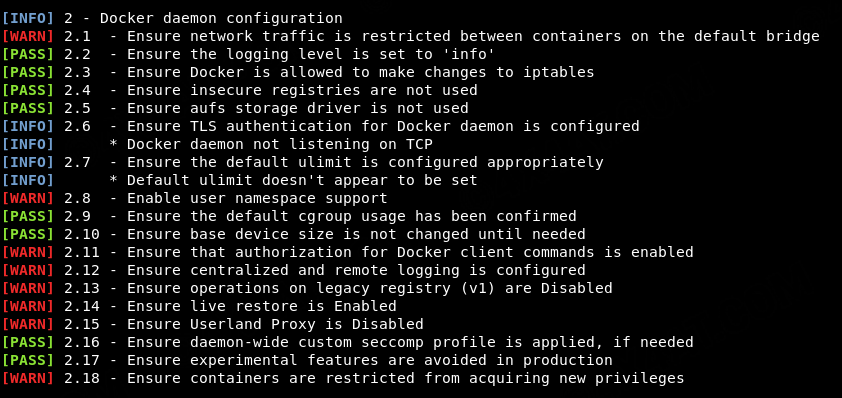
\includegraphics[width=15cm]{figuras/dockerBench.png}}
\caption{Saída parcial da execución da ferramenta \textit{Docker bench tool}}
\label{dockerBench}
\end{figure}


\section{Boas prácticas}

Hai unha serie de boas prácticas na emprega e configuración de entornos baseados en contedores aceptados pola industria. Moitos deles xa foron abordados ao longo deste documento, como poden ser:

\begin{itemize}
    \item \textbf{Principio de manter só o esencial:} cómpre reducir o número de binarios e servizos correndo dentro dos contedores, reducindo así as posibilidades de que un ataque teña lugar, ao limitar o número de vulnerabilidades existentes dentro dos contedores. Se queremos coñecer os paquetes instalados e o seu estado, podemos facer emprega de xestores de paquetes como poden ser {\tt dpkg}, tal e como amosa a figura \ref{dpkgl}.
    
    \begin{figure}
    \centerline{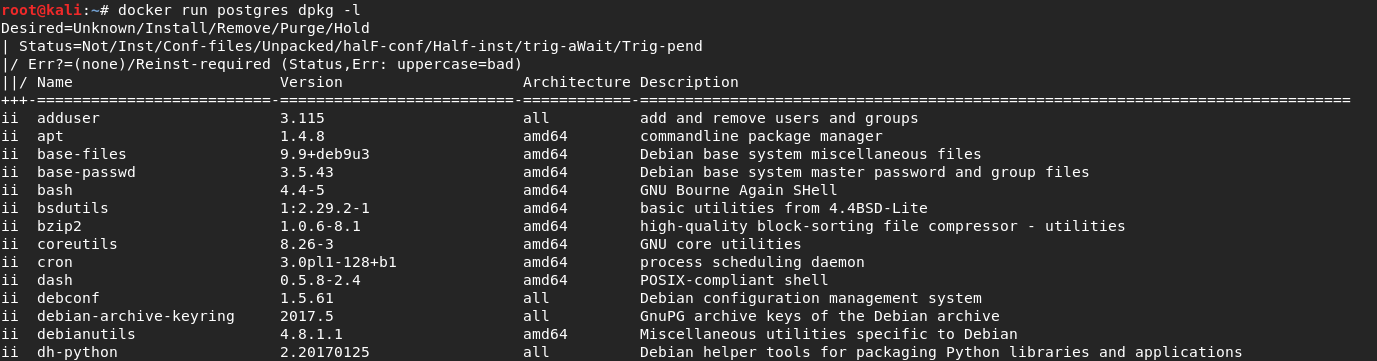
\includegraphics[width=15cm]{figuras/dpkgl.png}}
    \caption{Mostra de paquetes e versións nun contedor Docker con PostgreSQL 9.6}
    \label{dpkgl}
    \end{figure}
    
    \item \textbf{Empregar sistema de só lectura:} os sistemas de ficheiros son unha importante fonte de ataque por parte dos intrusos non desexados. Empregando un sistema de só lectura dentro dos contedores é posíbel parar certos tipos de ataques, como a subida de scripts maliciosos ou a sobreescritura de datos sensíbeis. Sempre que sexa posíbel, debemos empregar sistemas de só lectura nos contedores. Isto tamén é aplicábel aos volumes externos aos que estean conectados os contedores.
    
    \begin{lstlisting}[,caption={Proba de escritura en contedor de só lectura}]
docker run --read-only ubuntu touch proba
touch: cannot touch 'proba': Read-only file system
    \end{lstlisting}
    
    \begin{lstlisting}[,caption={Proba de escritura en sistema compartido de só lectura}]
docker run -v /root/Downloads/:/Downloads:ro ubuntu touch /Downloads/proba2
touch: cannot touch '/Downloads/proba2': Read-only file system
    \end{lstlisting}
    
    \item \textbf{Limitar as chamadas ao \textit{kernel}:} posto que contedores e máquina anfitrioa comparten \textit{kernel}, esta resulta unha proposta moi interesante, posto que un ataque exitoso sobre o \textit{kernel} do sistema podería ter serias implicacións non soamente no propio contedor, senón tamén noutros contedores e na propia máquina anfitrioa. Unha posíbel solución podería pasar pola emprega de sistemas enfocados na seguridade como \gls{SELinux}, nos que é posíbel limitar as chamadas ao sistema que un contedor pode facer.
    
    \item \textbf{Limitar os recursos:} para evitar posíbeis ataques de denegación de servizo é importante limitar os recursos que un contedor pode empregar. Estas limitacións poder vir dadas pola propia tecnoloxía de contedorización ou facer uso de sistemas externos baixo diversos criterios de clasificación.
    
    \item \textbf{Reducir as vulnerabilidades existentes nas imaxes:} coa a axuda de ferramentas externas é posíbel descubrir as vulnerabilidades que posúen as imaxes dos nosos contedores. Tendo coñecemento das mesmas podemos aplicar medidas para reducilas, por exemplo actualizando á última versión as librarías a empregar.
    
    \item \textbf{Manter actualizadas as tecnoloxías de virtualización:} a medida que as tecnoloxías de virtualización actualízanse incorporan novas e mellores medidas de seguridade. É importante manter o sistema actualizado para obter ditas melloras, sobre todo cando é lanzada algunha versión enfocada na revisión da seguridade do sistema, como supuxo Docker 1.10 coa introdución de espazos de nomes para usuarios.
    
    \item \textbf{Tratamento adecuado de información confidencial:} cando traballamos con certas aplicacións é posíbel que precisen facer uso de información confidencial, tal como contrasinais (por exemplo, para realizar accesos a bases de datos). Se un atacante logra ter acceso a esta información, tamén gañará o acceso a estes servizos, polo que é importante manter segura esta información. Debemos evitar facer emprega das variábeis de entorno para almacenar esta información, xa que son doadamente accesíbeis e amplamente empregadas. No seu canto, esta información pode ser almacenada en ficheiros no interior de volumes externos aos que só o usuario adecuado teña permisos de acceso. Para incrementar a seguridade, ditos volumes deberían ser de só lectura, evitando que alguén puidera modificar dita información.
    
    \item \textbf{Non dar acceso a directorios perigosos da máquina anfitrioa:} algúns contedores precisaran acceso a directorios especiais como {\tt /proc}, {\tt /dev}, etc. Normalmente, estas montaxes son precisas para realizar algunha funcionalidade especial do contedor, non obstante, debemos asegurarnos de comprender por que e como certos procesos queren acceder a información privilexiada. Habitualmente, expor estas rutas privilexiadas con permisos de só lectura debería abondar, polo que non debemos outorgar privilexios de escritura sen nos preguntar por que.
    
    \item \textbf{Configurar ferramentas de xestión de \gls{OOM}:} para evitar posíbeis ataques de denegación de servizo, podemos facer uso de ferramentas que eviten a sobreemprega destes recursos do sistema, como pode ser a memoria. Algunhas tecnoloxías, como Docker, xa incorporan o seu propio ``\gls{OOM} \textit{killer}'', mais existe a posibilidade de configurar un xestor externo.
    
    \item \textbf{Configurar o \textit{socket} de Docker de xeito seguro se é precisa unha conexión en rede:} por defecto, Docker execútase a través dun \textit{socket} Unix non conectado á rede, pero tamén é posíbel empregar un socket HTTP no caso de querer que dita tecnoloxía funcione en rede. Neste caso, é preciso configurar unha serie de parámetros se queremos que a emprega de Docker en rede sexa segura, como a habilitación de TLS ou a configuración de certificados.
    
    \item \textbf{Establecer un sistema de detección de vulnerabilidades en imaxes:} cando traballamos con imaxes provintes de diferentes fontes corremos o risco de despregar sistemas que conteñan vulnerabilidades. Para miniaturizar este risco e coñecer o estado ao que pasará o noso sistema de despregar tales imaxes podemos facer uso de ferramentas que permiten a detección de vulnerabilidades. Estas ferramentas permitirán a identificación de vulnerabilidades antes de que o sistema sexa despregado, outorgándonos gran cantidade de información, segundo a cal poderemos actuar. Existen incluso ferramentas que se poden integrar nun proceso de despregamento no que non se permita a instanciación de contedores que conteñan certas vulnerabilidades.
    
    \item \textbf{Empregar mecanismos de validación de imaxes:} todas as tecnoloxías de contedorización estudadas posúen mecanismos para a validación das imaxes, conseguindo aumentar a seguridade do sistema ao permitirnos tratar só con imaxes fiábeis. Deberiamos empregar soamente aquelas imaxes cuxa procedencia sexa coñecida e fiábel.
    
    \item \textbf{Empregar mecanismos externos de seguridade:} a seguridade por capas é unha das mellores solucións que existen, posto que se unha das capas se ve comprometida, aínda existirán outras que manterán seguro ao sistema. Por isto, a emprega de solucións externas para a protección do noso sistema baseado en contedores poden ser moi interesantes. Unha das solucións externas máis soadas a día de hoxe é \gls{SELinux}.
    
    \item \textbf{Manter o sistema actualizado:} para obter as últimas actualizacións de seguridade cómpre manter o noso sistema ao día na medida en que isto sexa posíbel. Esta actualización afecta tanto á máquina anfitrioa como ao sistema interno de cada contedor individual.

\end{itemize}
